%------------------------------------------------------------------------------
%Description       : DDMoRe WP7.2.1 First Technical Specification for the Model
%                                   Repository Infrastructure - Proposed Design 
%Author            : Mihai Glonț <mglont@ebi.ac.uk>
%Organization      : EMBL-EBI
%                    Wellcome Trust Genome Campus
%                    Hinxton
%                    Cambridge
%                    United Kingdom
%------------------------------------------------------------------------------
\section{Proposed Design}
\label{proposedDesign}
\idea{Add general description of the topics covered in this section.}

\subsection{Use Cases}
\label{useCases}
The aim of this section is to describe how each of the aforementioned stakeholders interact with the system. Each such interaction is called a \gls{usecase}, while the user performing it is known as an \gls{actor}. The use cases listed in Figure~\ref{fig:useCases} only consider the main actors that are involved, hence Administrators are not mentioned in any model-related use cases, in spite of the fact that they do have the authority required to perform any action. 

\begin{figure}[htb]
\centering
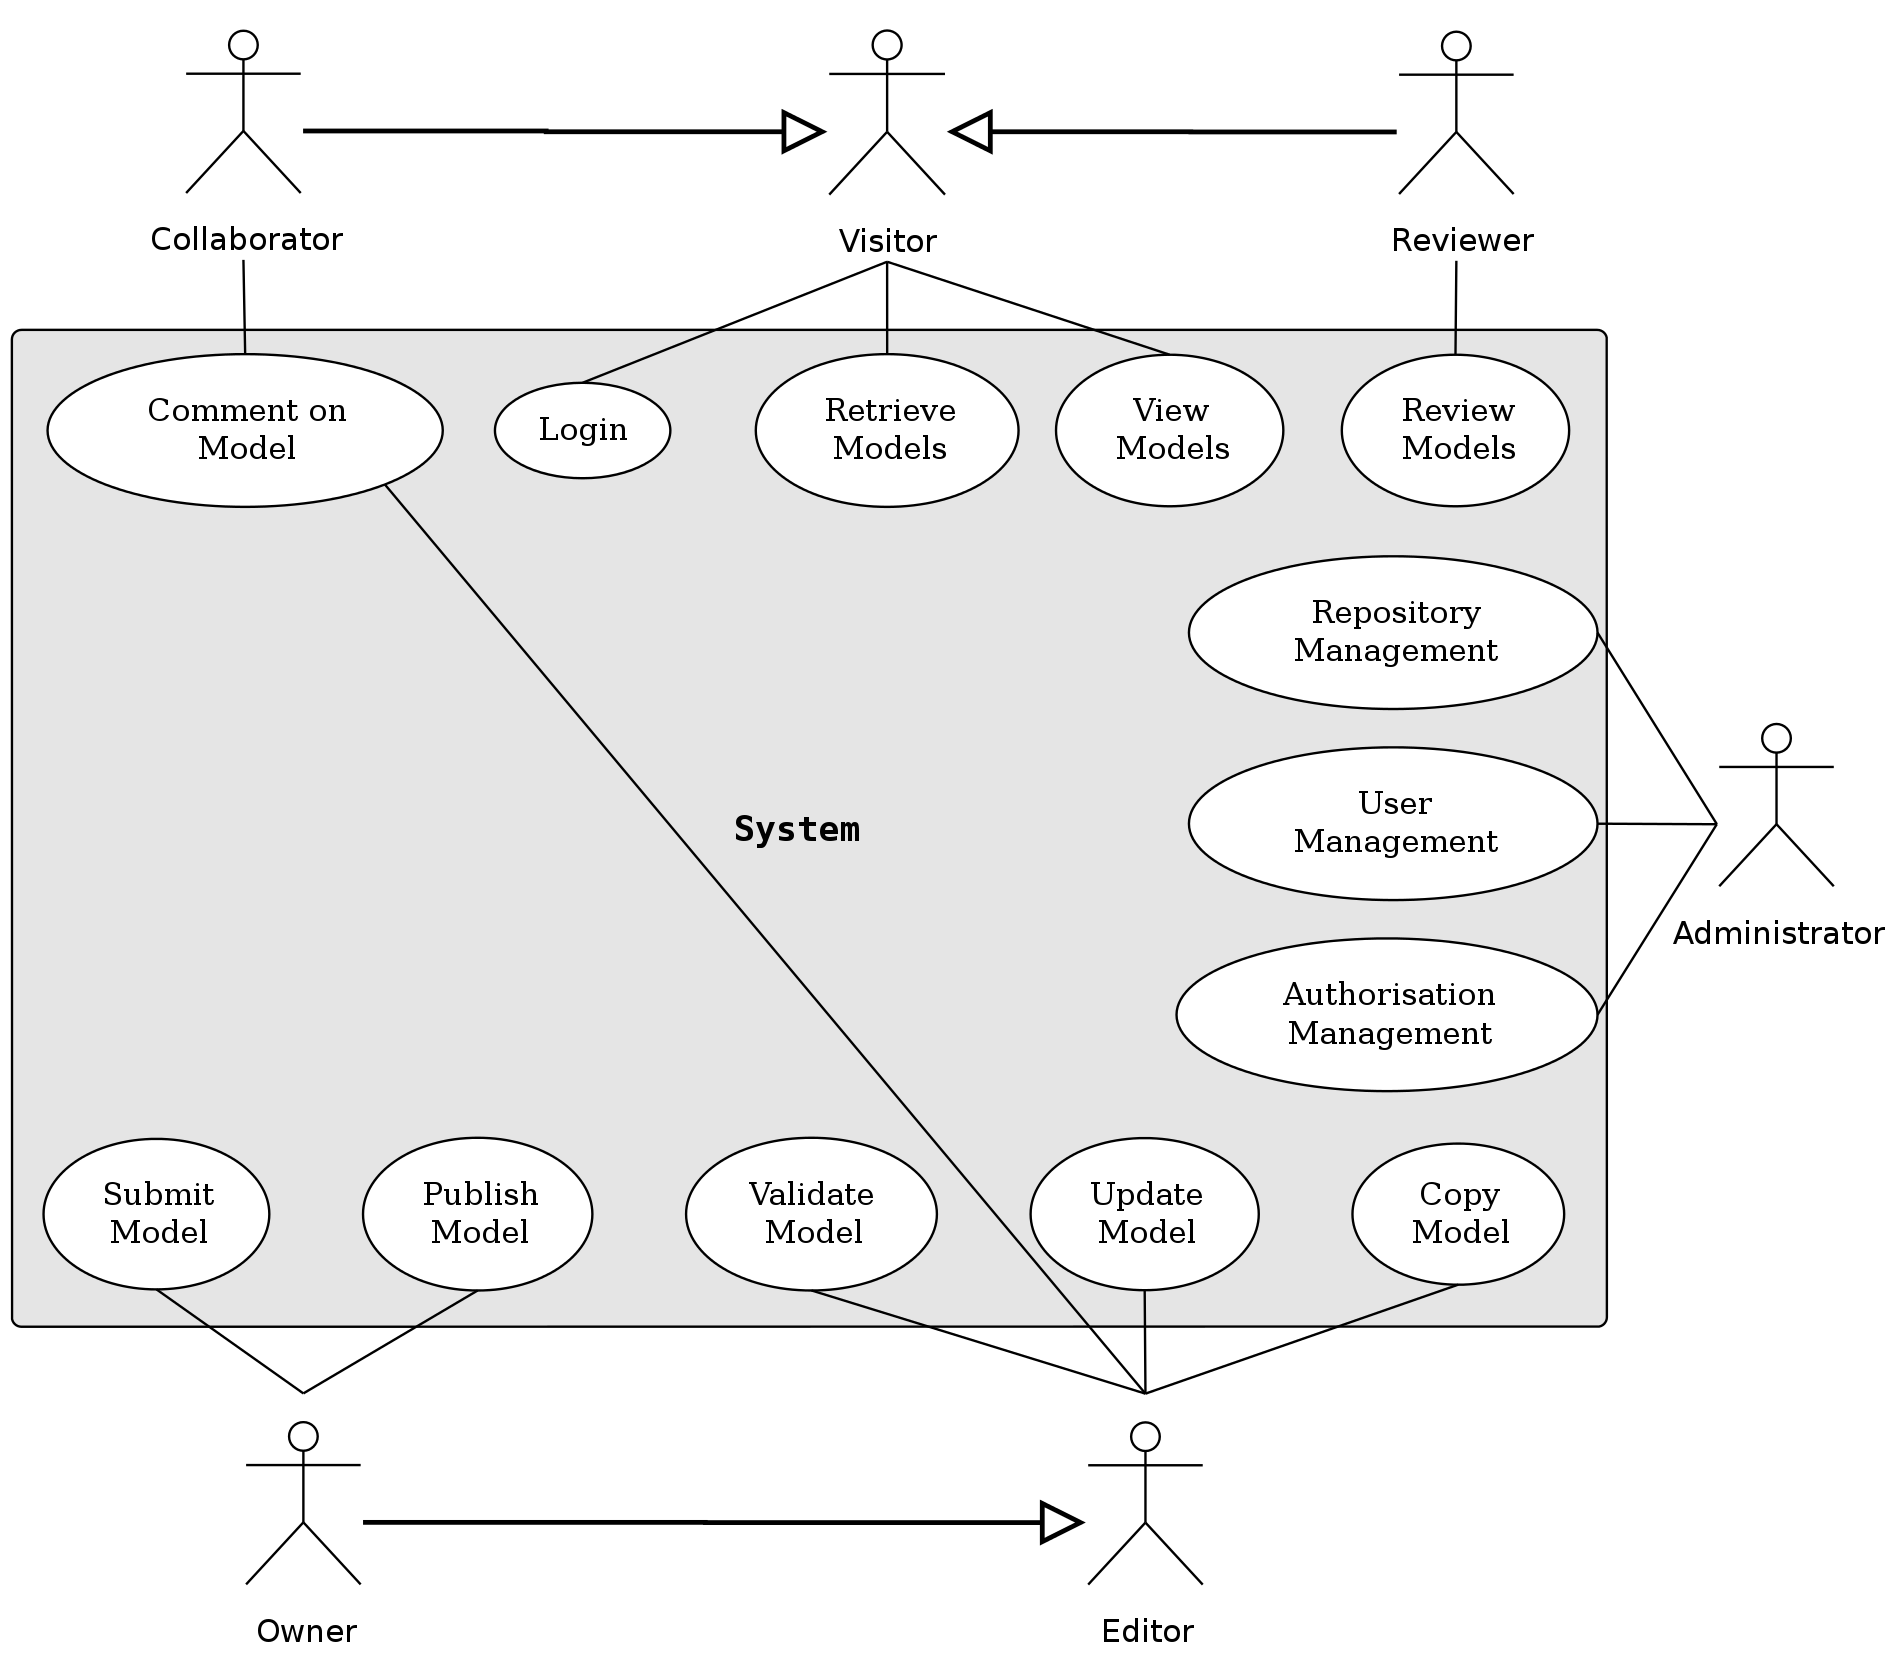
\includegraphics{img/UseCases}
\caption{Diagrammatic representation of the system's scope.}
\label{fig:useCases}
\end{figure}

\subsection{Proposed Work flows}
\label{workFlows}
\idea{UML Activity and Sequence diagrams should go in the appendix, should there be many of them. This section should only discuss them.} 

\subsection{Software Infrastructure}
\label{softwareInfrastructure}
\idea{Add UML Deployment diagram showing the link between a DB server, a Web server (possibly a servlet container behind an HTTP server) and a folder under version control.}

\subsection{Mock-ups}
\label{mockUps}
\idea{General UXD comments behind the look and feel of the pages. Actual mock-ups should be in the appendix. Landscape page format might be required for this part.}

%------------------------------------------------------------------------------
%Description       : DDMoRe WP7.2.1 First Technical Specification for the Model
%                                   Repository Infrastructure - Web Services
%Author            : Mihai Glonț <mglont@ebi.ac.uk>
%Organization      : EMBL-EBI
%                    Wellcome Trust Genome Campus
%                    Hinxton
%                    Cambridge
%                    United Kingdom
%------------------------------------------------------------------------------
\subsection{Programmatic Interaction with the \ddmore Model Repository}
\label{webServices}
\idea{This section is dedicated to programmatic access to and manipulation of models. It should provide a diagrammatic representation of the envisaged architecture along with the considerations behind it. A discussion on the integration with other software systems within \ddmore should also be included.}



\subsection{Security Considerations}
\label{securityConsiderations}
\idea{Exclude data centre, hardware and network security aspects from the scope of this document. Recommend running the HTTP server and the servlet container as different users with limited privileges. Beware that the user running the servlet container needs write access to the folder storing models. Discuss the need to protect the metadata directory within the folder where the models are stored (e.g. .git, .hg, .svn), as access to them outside the designated protocol - i.e. the web interface - should be prohibited.}

\subsection{Licence}
\label{licence}
The code for the \ddmore Model Repository will be hosted on SourceForge and released under a GPL-compatible licence. This licence does not apply to the models stored in either the public Repository or any private instance of it. 
